\documentclass[font=default]{mpltx}
\usepackage{bm, ctex}
\usepackage{subfigure}
\usepackage{multirow}
% 以下至 \begin{document} 都仅是本文件为了方便额外定义的命令, 写报告时不需要.
\hypersetup{colorlinks=false}% 超链接带颜色
\usepackage{xcolor}
% 以上是本文件为了方便额外定义的命令, 写报告时不需要.
\linespread{1.5}
\begin{document}

\title{实时高温电阻测量研究${\rm MgB_2}$相变} % 切合报告内容, 简短明确, 可以不同于讲义
\author{MaskedName} % 这里 \emailphone 一定要紧跟在 \author 后方
\emailphone{MyMail@stu.pku.edu.cn}{Tel}
% 如果改用 \email 则仅需要邮箱参数
\affiliation{北京大学物理学院\quad 学号: StudentID}
\date{\zhdate{2023/11/15}}
\begin{abstract}
本实验旨在研究硼(B)和镁(Mg)在高温条件下进行固相反应生成二硼化镁(MgB$_2$)的过程。首先,我们制备了硼-镁前驱体块材样品,并通过高温电阻法进行测量,以监测样品在烧结过程中的电阻变化。通过分析加热、保温和降温三个过程中样品电阻与温度的关系,我们能够确定电阻骤降对应的固相反应起始温度。此外,对实验过程中的其他细节进行了深入讨论。
\end{abstract}

\keywords{实时高温电阻法,相变,固相反应,MgB$_2$}

\maketitle

\section{引言}
新材料在人类社会发展的过程中起着至关重要的作用,新材料的形成过程总是伴随着相变。研究相变的方法有很多,如热分析法、差热分析法、中子衍射和实时高温电阻率法等等。其中“实时高温电阻率测量法”相比起来仪器设备比较简单、操作方便、运行成本比较低。本实验中我们使用实时高温电阻率测量法来观测二硼化镁(MgB$_2$)块材的相变过程。

MgB$_2$早在20世纪50年代就被人们所熟知,在2001年,这种材料被发现接近甚至突破了传统BCS理论预言的简单金属化合物临界温度的极限值$T_c=39$ K(Akimitsu等人),这引起了各国科学家们的兴趣。MgB$_2$的临界温度$T_c$几乎是其他同类型超导体临界温度的两倍,具有优良的超导性质。而其晶体结构导致MgB$_2$具有较小的各向异性,相干长度较长,超导电流不受晶界连通性的限制。这些优点使得MgB$_2$在理论研究方面有着很大意义的同时,也在各个材料领域有着很广泛的应用和良好的前景。

本实验中我们通过镁粉和硼粉压制成镁硼混合物样品,并在真空中通过高温相变制备MgB$_2$(在氩气环境中MgB$_2$的相变温度更低\cite{Feng},但是为了简单操作起见,我们还是选择在真空中烧制MgB$_2$样品)。期间,我们使用实时高温电阻率测量法研究MgB$_2$的相变过程,我们将通过对烧结过程中MgB$_2$块材的电阻进行实时测量,从而分析烧结过程中发生的物理现象。通过从硼粉到镁粉制备出MgB$_2$块材的整个过程,我们可以大致了解制备大块样品的一般工艺;通过对于烧结过程的分析,我们可以对相变的本质有更进一步的理解。

\section{理论\cite{book}}
\subsection{相变}
一般来讲,在物理学中,相是指在热力学系统中的一个区域,该在该区域内,材料的所有物理性质基本上是均匀的。由此可以将材料分成两类,一类是只包含一个相的材料,称为单相材料;一种是包含多个相的材料,称为复相(多相)材料。

相变就是在一定的外界条件下,系统由一个相变为另一个相。一般来说,物质在相变前后的物理性质或者化学成分会发生一定的变化。而按照相变时的热力学参量变化特征,相变可以分为一级相变和高级相变(也叫连续相变)。热力学体系的的化学势(或者其他热力学函数)通常依赖于温度、体积和压力,化学势在相变点也是连续的,但是其导数可能会有突变。如果在某个相变点,体系的化学势的一阶导数发生了突变,也就是体积或者熵发生了突变,那么这种相变就称作一阶相变,单位体积或者熵的改变量为
\begin{equation}
  \begin{aligned}
    \Delta v&=\left(\frac{\partial\mu}{\partial p}\right)_{T_0^+}-\left(\frac{\partial\mu}{\partial p}\right)_{T_0^-},\\
    \Delta s&=\left(\frac{\partial\mu}{\partial T}\right)_{T_0^-}-\left(\frac{\partial\mu}{\partial T}\right)_{T_0^+}.
  \end{aligned}
\end{equation}
反之,如果化学势的一阶导数连续,而高阶导数发生了突变,那么这种相变就称作高阶相变(也称为连续相变,化学势的几阶导数发生突变就是几阶相变)。目前为止我们最高也只在实验上观察到二阶的相变,二阶相变发生时,系统的体积和熵不会发生突变,但是定压比热、定压膨胀系数和等温压缩系数会发生变化。

新材料的形成往往伴随着相变,不同材料可以在一定条件下发生反应(也就是相变)生成新的材料。本实验就是通过硼粉和镁粉之间的固-固反应来获得MgB$_2$新相的。
\subsection{影响固相反应的因素}
从热力学的角度考虑,两种物质能发生反应,前提条件是反应朝着吉布斯自由能减少的方向进行。也就是反应前后$\Delta G<0$。自由能的减少越多($\Delta G$负值越大),反应进行的倾向就越大。

接下来考虑动力学的部分,也就是影响反应速率的部分。反应速率由如下几个因素共同影响:(a)反应物的颗粒度和均匀性。反应物的颗粒度越小,比表面积越大,其反应速率就越大;反应物越均匀,体系中能发生化学反应的面积就越大,反应速率越大。(b)反应温度。温度越高,粒子动能越大,参与反应的粒子扩散能力更强,反应速率也就越大。(c)环境气氛和固体压力。气氛的存在能够使得容易气化得反应物得原子逸出率降低,从而让不同原料之间的反应充分进行。在合适的压力下,反应物粉粒之间能够更加紧密的接触,从而增大反应速率。
\subsection{样品烧结的过程}
下面就本实验涉及到的MgB$_2$样品烧结的过程进行讨论。

因为固相材料一般在化学上是不活泼的,所以反应一般在高温下进行。当参与反应的粒子半径不同的两种原料A、B的粉体以\autoref{fig:mixed_particles} 的方式被均匀混合后,由于A、B的粒径不同,它们混合后将是以小颗粒的粉粒包围大颗粒的粉粒的方式接触。本实验中,我们用的硼粉颗粒度是1 $\mu$m,镁粉的颗粒度在0.1 mm的量级。在这种镁的颗粒度大,硼的颗粒度小的情况下,在两种粉均匀混合后,是硼粉均匀包住镁粉的颗粒。这样,被压成的母体材料整体表现出来的就是非金属性:在室温下材料的电阻很高,随着温度的升高,材料的电阻率不断下降。但是当温度升高到一定程度,化学反应开始比较明显地发生,MgB$_2$晶粒大量生成,那么这个时候样品的电阻率就会急剧下降。因此我们可以通过实时测量被烧结的固体材料在高温烧结过程中电阻率随温度的变化来判断相变发生的温度窗口。

值得注意的是,如果镁颗粒和硼颗粒的半径不同,那么实验测量出来的结果就会不一样,不同镁粒子半径、相同硼原子(约1 $\mu$m)下,固体材料电阻率随温度的变化如\autoref{fig:size_effect}所示。
\begin{figure}[h]
  \centering
  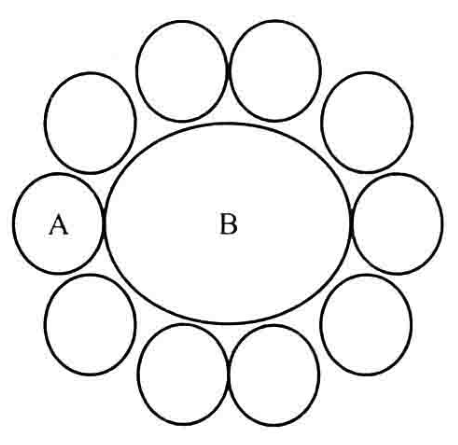
\includegraphics[width=0.25\linewidth]{fig/mixed_particles.png}
  \caption{粒子半径不同的两种粉体材料均匀混合后参与反应的模式(在本实验中,A代表硼原子,B代表镁原子)}
  \label{fig:mixed_particles}
\end{figure}

\begin{figure}[h]
  \centering
  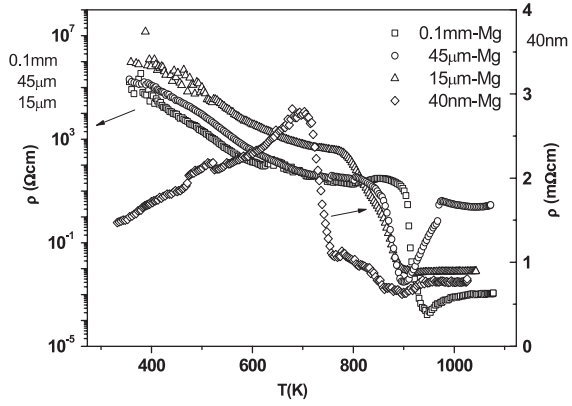
\includegraphics[width=0.55\linewidth]{fig/size_effect.png}
  \caption{不同镁粒子半径、相同硼原子(约1 $\mu$m)下,固体材料电阻率随温度的变化(图片来自\cite{Zhuang})。}
  \label{fig:size_effect}
\end{figure}
\section{实验内容}
\subsection{样品的制作}
本实验使用镁粉和硼粉压制制作混合物样品。设置总质量约为 1 g,按取二者的物质的量之比为1.2:2确定硼粉和镁粉的质量(考虑到镁在高温易升华,镁的原子量要比理论上略多一些),计算得到镁粉约0.53 g,硼粉约0.47 g。用电子天平称量此质量的硼粉和镁粉,并放入玛瑙研钵中充分研磨,使二者充分混合。

接着,根据实验要求组装所需的模具(模具采用可拆卸的模具,具体详见实验课本\cite{book})。将混合均匀的粉末倒入模芯组块的凹槽内。剪下两段长度合适的钼丝作为引线,用夹线夹片中间的凹槽夹好引线,一侧露出约3 mm的长度。然后,将引线压入装满粉末的模具凹槽内,注意将钼丝的上半段弯入夹线夹片的凹槽内,以防止压机工作时将钼丝压断。

在模具上面放上护垫后,将其放入压机中。然后,施加10吨的压力进行压制。维持该压力2分钟后,撤去压力,并将模具退出来,就可以得到压制成型的样品块体材料。
\subsection{样品的烧结}
样品压制完成之后,将样品的引线套上绝缘的陶瓷套管以防止短路,随后将样品放入样品烧结盒中,并用盖子盖住。由于本实验中我们使用的镁粉颗粒比较大而硼粉颗粒较小,根据上面的分析,在发生相变前,样品应呈现非金属性,电阻是很大的,所以本实验中我们只需要使用二线接法将引线接入反应舱的接线柱。

随后将钟罩合上,打开水泵通入冷凝水,接通电源对其用机械泵抽真空。反应舱的压强抽到一个较低的水平后(实际实验中降至约10 Pa时),按照程序设定的升温、保温、降温三阶段进行温度设定(实验室已经提前设置好),并实时监测样品电阻与温度的值。本实验使用虚拟仪器Labview直接控制系统进行测量和数据采样,在启动测量装置之后,只需要耐心等待就可以得到想要的数据。

\section{实验结果与分析}
利用Labview进行测量,得到的测量结果如\autoref{fig:lnR_T_T_t} 所示。温度有三个变化区间:升温、保温和降温。在升温之前,样品呈现非金属性,阻值较高,且随着温度的升高组织不断降低。在温度升高到一定程度时,样品的电阻突变到一个很小的值,说明此时发生了相变,生成了MgB$_2$。而之后降温的时候,电阻基本上维持在一个值不变,说明这个相变是不可逆的。

为了更好的分析整个相变过程,我们将分别研究在不同温度的变化区间内,电阻随温度的变化。
\begin{figure}[h]
  \centering
  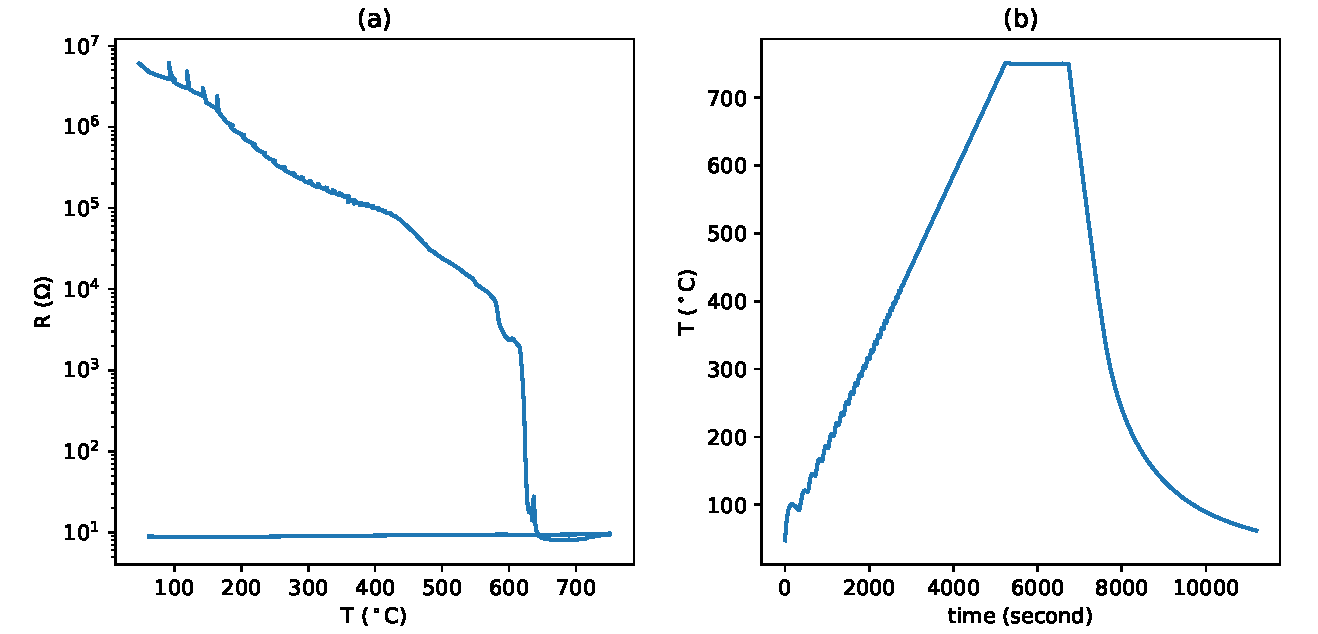
\includegraphics[width=0.9\linewidth]{fig/lnR_T_T_t.pdf}
  \caption{实时高温电阻率测量法测量MgB$_2$相变过程的数据。(a)电阻$R$随温度$T$的变化图像,由于本实验中电阻变化比较大,所以这里$R$轴使用对数坐标;(b)温度$T$随时间$t$的变化图像,从中可以看到实验的三个过程:升温、保温和降温。}
  \label{fig:lnR_T_T_t}
\end{figure}
\subsection{升温阶段}\label{sectionA}
升温过程的$R-T$曲线如\autoref{fig:lnR_T_up} 所示($R$轴选用对数坐标轴),这和\autoref{fig:size_effect} 中0.1mm-Mg的曲线是吻合的。可以看到原先的混合物质具有相当大的电阻(M$\Omega$级别),并且随着温度升高逐渐降低,在大约600 $^\circ$C时发生向下的突变,说明此时发生相变,从绝缘体转变到导体,说明此时MgB$_2$已经形成。

对$\log R-T$曲线求微分(用差分代替),得到${\rm d}(\log R)/{\rm d}T-T$曲线如\autoref{fig:dlnRdT_T_up} 所示。由于在升温过程中,出现了一些电阻跳变的点(可能是由于导线接触不良导致的),所以在红色阴影部分会出现一些奇异的点,但是若我们将这些奇异点去掉,就可以发现在600 $^\circ$C之前,微分值的波动还是相对较小的。而在610 $^\circ$C\textasciitilde650 $^\circ$C这个区间,${\rm d}(\log R)/{\rm d}T$值得波动是很大的,说明在这个时候发生了相变。因此我们可以认为MgB$_2$的成相温区就是610 $^\circ$C\textasciitilde650 $^\circ$C。
\begin{figure}[h]
  \centering
  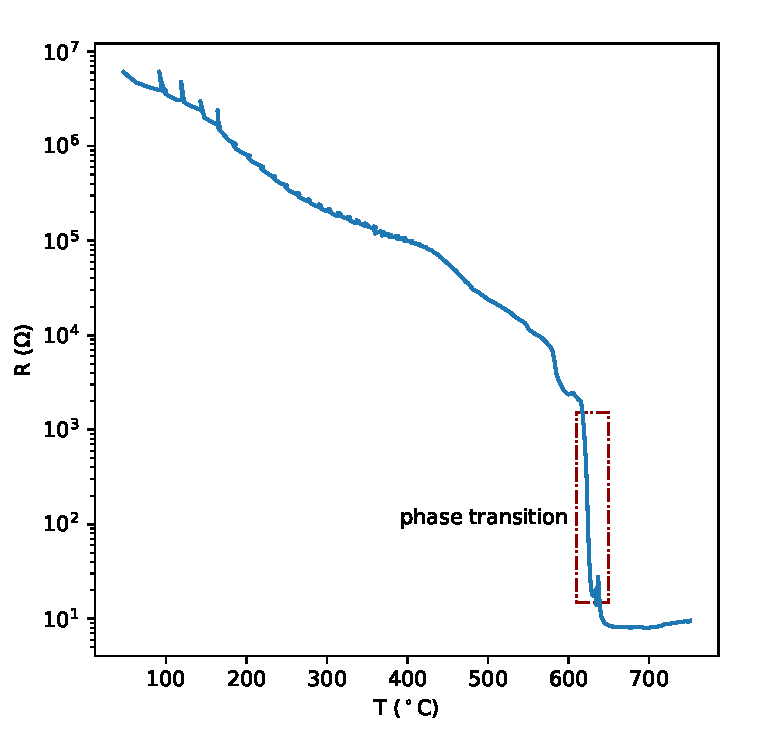
\includegraphics[width=0.5\linewidth]{fig/lnR_T_up.pdf}
  \caption{升温过程中电阻$R$随温度$T$的变化,$R$轴使用对数坐标。在图中用红框圈出的部分是电阻在升温过程中骤然下降的部分,说明在这个区间发生了相变。}
  \label{fig:lnR_T_up}
\end{figure}
\begin{figure}[h]
  \centering
  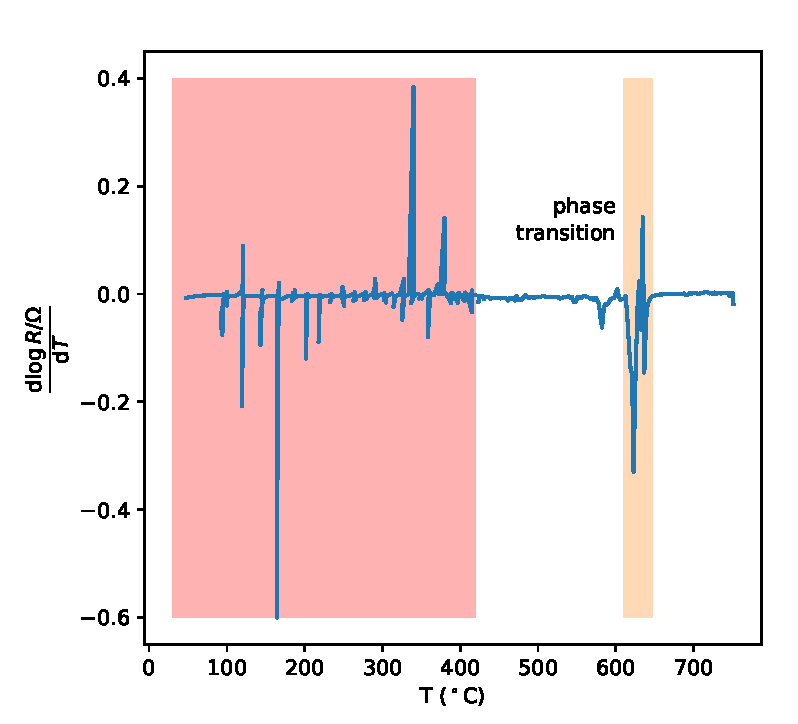
\includegraphics[width=0.53\linewidth]{fig/dlnRdT_T_up.pdf}
  \caption{升温过程中的${\rm d}(\log R)/{\rm d}T-T$曲线。橙色阴影部分是微分值跳变最大的部分,说明这是发生相变的部分(610 $^\circ$C\textasciitilde650 $^\circ$C)。由于在升温过程中,出现了一些电阻跳变的点(可能是由于导线接触不良导致的),所以在红色阴影部分会出现一些奇异的点,但是若我们将这些奇异点去掉,就可以发现在600 $^\circ$C之前,微分值的波动还是相对较小的。}
  \label{fig:dlnRdT_T_up}
\end{figure}
\subsection{保温阶段}
在保温阶段,温度控制在在750 $^\circ$C附近,作出电阻随时间的$R-t$图像如\autoref{fig:R_t_const} 所示。虽然在不同地方电阻值会有一些小波动,但是总体来说,电阻的变化是不大的(约在9.46 $\Omega$到9.83 $\Omega$之间变化)。这个波动可能有两个来源:1.虽然程序控制下温度应该是恒定的,但是由于加热方式的原因(通过不断地通电断电来控制温度),温度事实上还是会有一定的波动,这也导致了电阻的波动。2.在样品反应充分之后,还有一定量的镁或者硼残留下来,这些残留下来的单质在750 $^\circ$C下会有一定的逸出,这也可能对样品的电阻产生影响。
\begin{figure}[h]
  \centering
  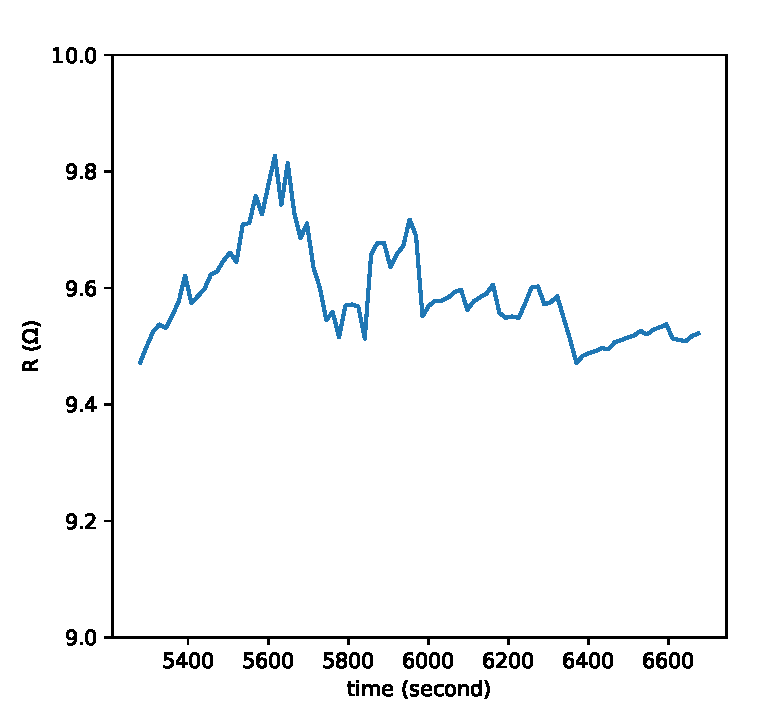
\includegraphics[width=0.5\linewidth]{fig/R_t_const.pdf}
  \caption{在保温阶段电阻$R$随时间$t$的变化。这个阶段电阻相对较小,而且波动也不大(约在9.46 $\Omega$到9.83 $\Omega$之间波动)。}
  \label{fig:R_t_const}
\end{figure}
\subsection{降温阶段}
降温阶段的$R-T$曲线如\autoref{fig:lnR_T_down} 所示($R$轴选用对数坐标轴)。可以看到,样品在降温阶段电阻随温度降低而存在缓慢地降低,这是MgB$_2$样品金属性的体现。但是电阻实际上下降的幅度并不是很大,说明我们制作的样品是相对比较纯净的。当然这个实验由于我们使用的是二接线法进行测量,测量结果难免会受到接触电阻比较大的影响。为了得到更加精确的结果,可以采取严格的四线法线路来测量电阻。
\begin{figure}[h]
  \centering
  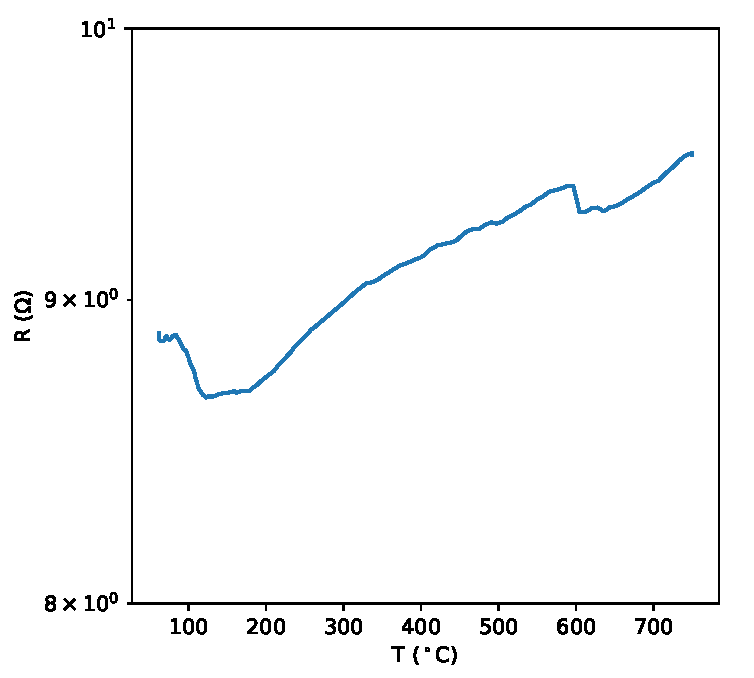
\includegraphics[width=0.5\linewidth]{fig/lnR_T_down.pdf}
  \caption{降温过程中电阻$R$随温度$T$的变化,$R$轴使用对数坐标。}
  \label{fig:lnR_T_down}
\end{figure}
\section{结论}
本次实验采用硼和镁的固相反应成功合成了二硼化镁(MgB$_2$)相,通过对样品电阻随温度的变化,深入研究了该二元体系的固态相变过程。由于金属性的MgB$_2$是从绝缘体状态的“硼包镁”中生成的,因此在相变时体系电阻会迅速降低。实验结果表明,固相反应的临界温度约为610 $^\circ$C。此外,我们对样品在升温-保温-降温全过程中的电阻变化进行了详细分析,探讨了不同曲线趋势所代表的不同相以及它们对应的理论。同时,对实验结果与理论之间的差异进行了简要分析,以揭示可能导致差异的原因。通过实时高温电阻率测量法对MgB$_2$块材的相变过程进行研究,我们不仅深刻理解了MgB$_2$的相变特性,还获得了关于烧结过程中发生的物理现象的深层见解。这一实验为我们提供了制备大块样品的通用工艺,并对相变的本质有了更深层次的认识,为进一步探索相关领域的研究奠定了基础。

\begin{acknowledgments}
特别感谢张焱老师在实验过程中的指导。感谢刘新阳学长协力完成了本实验。
\end{acknowledgments}

\begin{thebibliography}{}
  \bibitem{Feng} Q. Feng, X. Chen, Y. Wang, X. Wang, G. Xiong, and Z. Gao, “In situ resistance measurement of superconducting MgB2 in flowing argon atmosphere,” \textit{Phys. C Supercond.}, vol. 386, pp. 653–656, Apr. 2003, doi: 10.1016/S0921-4534(02)02184-6.
  \bibitem{book} 吴思诚, 荀坤. 近代物理实验(第四版). 北京: 高等教育出版社, 2015.
  \bibitem{Zhuang} C. Zhuang et al., “The size effect of raw materials on the phase formation of polycrystalline MgB2,” \textit{Supercond. Sci. Technol.}, vol. 20, no. 12, p. 1125, Sep. 2007, doi: 10.1088/0953-2048/20/12/007.
\end{thebibliography}
  
\clearpage % 附录前另起一页
\appendix % 附录开始
\section{思考题}
\subsection{超导材料由正常态转变为超导态时发生的相变与本实验中发生的相变有何区别?例如这两种相变是同一级别吗?为什么?}
超导材料由正常态转变为超导态时发生的相变是二级相变,其化学势的一阶导数在相变中不发生变化,也就是说二级相变在发生时是不会产生吸放热的现象的。但是本实验中发生的相变是一个化学反应,其必然发生了一定的焓变,也就是有吸放热产生。因此本实验发生的相变是一个一级相变。

\subsection{如何保证镁粉和硼粉的均匀混合以及${\rm MgB_2}$前驱体与引线处于良好的接触状态?}
首先我们需要保证两种粉末充分混合,为此我们需要一定长度的研磨时间,直到混合样品的颜色均匀。在研磨的时候力气不应该太大,以防止样品结块,阻碍更进一步的混合。为确保引线和前驱体充分接触,需特别注意将端点尽可能放置于样品中心位置。为防止端点移动,必须利用夹片来确保引线位置的牢固。
\subsection{为什么在烧结样品时要保证真空钟罩内的压强必须小于一个大气压?}
首先,为确保实验的成功进行,必须确保反应环境尽可能真空,以防止反应环境中残留的气体分子与镁粉和硼粉等反应前体发生不必要的反应。此外,过高的温度可能导致气体膨胀,从而破坏仪器的气密性,对仪器造成损害。最后,在实验过程中,会有少部分镁升华为气体,这就破坏了我们创造的固相反应体系,所以要将升华的镁不断抽走。因此,在实验过程中我们始终保持机械泵运行抽真空。
\subsection{为什么对硼包镁前驱体测得的高温$R-T$曲线的$R$值必须取对数?}
由于在升温前,样品的电阻值较高(达到M$\Omega$量级),远超过相变发生时的电阻值(在k$\Omega$ 量级)以及相变后的电阻值(在$\Omega$量级)。因此,如果在高温$R-T$曲线上不对电阻值取对数,绘制的图形在肉眼上将完全无法观测到电阻阻值的突变,从而难以准确确定固相相变的临界温度。
\subsection{根据得到的高温$R$-$T$曲线估计镁粉和硼粉的颗粒度关系,谁大谁小?}
在初始状态下,电阻较高,随着温度升高,样品电阻下降。这表明在这个阶段,样品体现出非金属性,即表现出硼的特性。因此,在样品中应该存在“硼包镁”的情况,即硼颗粒较小,而镁颗粒较大。
\subsection{${\rm MgB_2}$样品分别在真空环境和一定氩气环境下进行烧结,哪一个的成相温度高?}
在通入惰性气体后,处于氩气环境中能够有效防止易升华的镁粉颗粒向周围扩散,这有助于更顺利地进行固相反应,并且可能降低反应温度。因此,相比于真空条件下,氩气氛围下的成相反应在初始阶段可能具有更低的反应温度。

当然,也有前人做过的在流动的氩气环境下MgB$_2$的形成过程,实验结果和我们的理论推测是一致的\cite{Feng}。
\subsection{什么情况下必须用四引线法测量样品烧结过程中的$R$-$T$曲线?}
当测量电阻为小电阻时,接触电阻和引线电阻相对于所测量的电阻不可忽略,此时就必须用四引线法测量,以降低测量的误差。如果本实验的镁颗粒较小,而硼颗粒较大,那么混合物样品呈现的就是金属性,因此电阻很小。这种情况下我们就需要用四引线法测量样品烧结过程中的$R$-$T$曲线。
\subsection{试对得到的$R$-$T$或$\ln R$-$T$曲线求微分,从而求得${\rm MgB_2}$样品成相温区。}
参见\autoref{sectionA}的分析和\autoref{fig:dlnRdT_T_up}的结果。
\subsection{\autoref{fig:molding}(b)和\autoref{fig:demolding}(c)的底部所示的模芯垫块的区别是什么?}
在\autoref{fig:molding}(b)中,模芯垫块和模芯组块是相互紧密连接的,是在压片时的组装方式。而在\autoref{fig:demolding}(c)中,模芯垫块相较之前旋转了180$^\circ$,表示了在脱模时的组装方式。
\begin{figure}[h]
  \centering
  \setlength{\abovecaptionskip}{-0.2cm}
  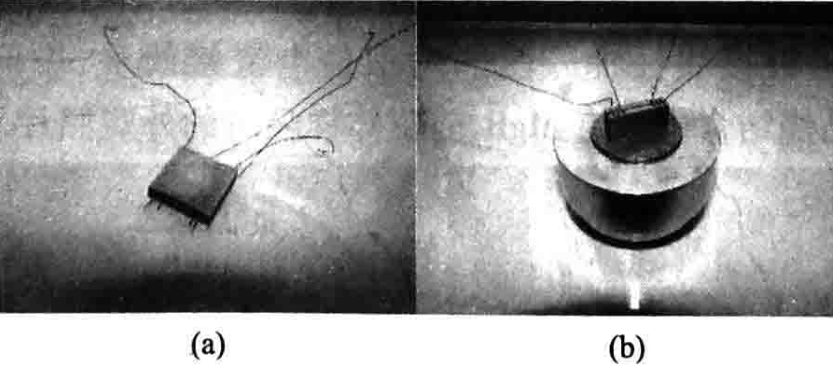
\includegraphics[width=0.47\linewidth]{fig/molding.png}
  \caption{(a)夹线夹片夹好引线后的状态;(b)夹好引线的夹线夹片插进粉料槽后的状态}
  \label{fig:molding}
\end{figure}
\begin{figure}[h]
  \centering
  \setlength{\abovecaptionskip}{-0.2cm}
  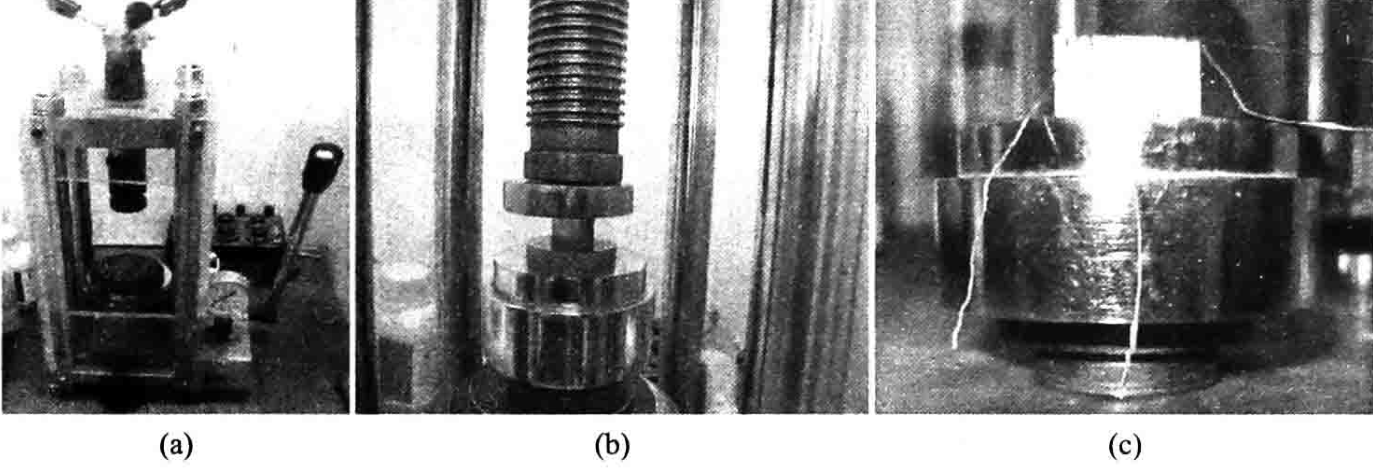
\includegraphics[width=0.7\linewidth]{fig/demolding.png}
  \caption{用小型压机压制样品及退模时模芯垫块所处的状态}
  \label{fig:demolding}
\end{figure}
\end{document}
